\documentclass[conference]{IEEEtran}

% ---------- Packages ----------
\usepackage{amsmath, amssymb, graphicx, cite, hyperref}
\usepackage{tikz}
\usetikzlibrary{calc,arrows.meta,positioning,fit,shapes.geometric}
\usepackage{pgfplots}
\pgfplotsset{compat=1.18}
\usepackage{siunitx}
\usepackage{balance}
\usepackage{microtype}

% ---------- Title ----------
\title{SkyEdge: Secure High-Altitude Drone Platform Integrating $H_\infty$ Control, Domestic Devices, and Advanced Mechanical Design}

% ---------- Author ----------
\author{
\IEEEauthorblockN{Shinichi Samizo}
\IEEEauthorblockA{Independent Semiconductor Researcher \\
Project Design Hub, Samizo-AITL \\
\textit{Email:} \href{mailto:shin3t72@gmail.com}{shin3t72@gmail.com} \\
\textit{GitHub:} \href{https://github.com/Samizo-AITL}{Samizo-AITL}}
}

\begin{document}
\maketitle

% ---------- Abstract ----------
\begin{abstract}
This paper presents a \emph{reference design} of \emph{SkyEdge}, a secure high-altitude unmanned aerial vehicle (UAV) platform integrating $H_\infty$ control, domestically manufactured devices, and a variable-pitch rotor system. The framework targets robust disturbance rejection, hardware-level security, and reliable operation up to 10\,000~m. Beyond an overview, we provide plant modeling, uncertainty description, mixed-sensitivity synthesis, gain scheduling for altitude variation, implementation details (timing and numeric), secure-boot/attestation flows with PQC, and a risk-driven evaluation plan with measurable KPIs. Applications include post-disaster communications, border monitoring, and environmental sensing.
\end{abstract}

\begin{IEEEkeywords}
UAV, robust control, $H_\infty$, gain scheduling, variable-pitch rotor, secure systems, TPM, PQC, high-altitude flight
\end{IEEEkeywords}

% =============================================================
\section{Introduction}
\IEEEPARstart{U}{AVs} enable persistent ISR, comms relay, and remote sensing. However, commodity systems degrade rapidly above 3--5~km due to (i) reduced air density $\rho(h)$ lowering rotor authority, (ii) sensor/actuator delays becoming non-negligible versus control bandwidth, and (iii) thermal/EMI margins shrinking in low-pressure cold environments. In parallel, globalized supply chains introduce opaque firmware and silicon provenance risks.

\textbf{Goal.} Build a domestically sourced, security-hardened quad-rotor platform sustaining closed-loop performance and thrust margin up to 10~km. Contributions:
\begin{enumerate}
  \item A mixed-sensitivity $H_\infty$ controller with structured uncertainty covering aerodynamics, inertia mismatch, and sensor delay, with altitude-aware gain scheduling.
  \item A secure device stack (65~nm FDSOI SoC, LDMOS ESC, TPM~2.0, PQC KEM) and a timed pipeline achieving $\le$1~ms control latency.
  \item A variable-pitch mechanism sized from thrust/torque models with fail-safe bias and health monitoring.
  \item A verification plan tying wind-tunnel, thermal-vacuum, and RF-jamming tests to quantitative KPIs and safety cases.
\end{enumerate}

% =============================================================
\section{Related Work}
PID dominates small UAVs for tuning simplicity but suffers overshoot/lag under gusts. Sliding-mode alleviates matched disturbances at the cost of chattering and sensor-noise amplification. $H_\infty$ offers worst-case guarantees via frequency shaping~\cite{zhou1996robust} but is less reported for 8--10~km operations. High-altitude fixed-wing/solar craft (Helios, HAPS) validate endurance but rely on bespoke airframes and imported avionics~\cite{nasahelios,jaxaHAPS}. On security, proprietary ciphers prevail; TPM-anchored boot and PQC standardization remain underused for UAV C2 links~\cite{pqcrypto2022}. Learning/MPC controllers~\cite{mpc2021,rluav2022} improve adaptation yet rarely integrate threat models or attestation.

% =============================================================
\section{Plant Modeling and Uncertainty}
We linearize about hover and decouple attitude channels. The roll channel is representative:
\begin{align}
\dot{x}&=Ax+Bu+Ew,\quad y=Cx + v, \nonumber\\
x&=\begin{bmatrix}\phi & p & \theta & q\end{bmatrix}^\top,
\end{align}
with $u=\Delta \tau_\phi$ (differential rotor torque), $w$ a gust/IMU-bias input, and $v$ measurement noise. The nominal $P(s)$ includes actuator and sensor dynamics:
\begin{align}
G_a(s)&=\frac{1}{\tau_a s+1},\ \tau_a\in[4,8]~\mathrm{ms}, \\
G_s(s)&=e^{-s\tau_s},\ \tau_s\in[0.2,0.6]~\mathrm{ms}.
\end{align}
Altitude $h$ affects thrust coefficient $C_T\propto \rho(h) \Omega^2$; we capture mismatch as multiplicative output uncertainty
$P_\Delta(s)=P(s)\big(1+W_\Delta(s)\Delta(s)\big)$,
$|\Delta|\le1$, with
\begin{equation}
W_\Delta(s)=\frac{0.3\,s/20+0.4}{s/200+1},
\end{equation}
covering $\pm(35$--$40)\%$ variations across 0--10~km including blade/Reynolds effects.

% =============================================================
\section{H$_\infty$ Synthesis and Scheduling}
\subsection{Mixed-Sensitivity Formulation}
We choose weights:
\begin{align}
W_1(s)&=\frac{s/M+\omega_B}{s+\omega_B\epsilon},\ \omega_B=12~\mathrm{rad/s},\ M=2,\ \epsilon=0.01,\\
W_2(s)&=\frac{s+\omega_U}{s/A+\omega_U},\ \omega_U=60~\mathrm{rad/s},\ A=1,\\
W_3(s)&=\frac{s}{\omega_H}+d,\ \omega_H=120~\mathrm{rad/s},\ d=0.02,
\end{align}
and minimize $\left\| \mathrm{diag}\{W_1S,\ W_2KS,\ W_3T\}\right\|_\infty$, $S=(I+PK)^{-1}$, $T=I-S$.
This enforces: low $|S|$ (gust rejection), bounded effort $|KS|$, and roll-off via $|T|$ (sensor noise).

\subsection{Altitude Scheduling}
Instead of full LPV, we schedule two parameters measured on-board:
air density ratio $\sigma(h)=\rho(h)/\rho_0$ and available rotor headroom $\eta=\Omega/\Omega_{\max}$.
We precompute three controllers $\{K_i\}_{i=0}^2$ for $(\sigma,\eta)\in\{(1,0.6),(0.6,0.75),(0.3,0.9)\}$ and interpolate
\begin{equation}
K(\sigma,\eta)=\sum_i \alpha_i(\sigma,\eta) K_i,\ \sum_i \alpha_i=1,\ \alpha_i\ge0,
\end{equation}
with rate-limited blending $\dot{\alpha}_i\le 2$~s$^{-1}$ to avoid bump.

\subsection{Observers and FDI}
A Kalman-like filter estimates $(\phi,p)$ with augmented bias states for gyro drift. Residuals $r_k=y_k-\hat{y}_k$ feed a $\chi^2$ change detector for sensor/ESC faults; persistent flags trigger FSM transitions and pitch-bias fail-safe.

% =============================================================
\section{Implementation Details}
\subsection{Timing and Numeric}
IMU at 1~kHz, ESC command at 2~kHz, attitude loop at 1~kHz. Measured end-to-end delay: sensor \SI{0.25}{ms}, compute \SI{0.40}{ms}, actuation \SI{0.20}{ms}, total \SI{0.85}{ms}. Controller runs in fixed-point Q1.15 for inner PIDs in ESC and Q3.29 for $H_\infty$ states; coefficients are range-checked to avoid overflow under worst-case steps. Jitter $<\!60~\mu$s with priority and lock-in cache.

\subsection{Resource Footprint}
$H_\infty$ roll/pitch/yaw filters: 18 states total, \textasciitilde14~kB RAM, \textasciitilde28~kB flash. TPM driver and PQC stack add \textasciitilde120~kB flash; Kyber encaps/decaps \textasciitilde2.8~ms on SoC.

% =============================================================
\section{Security Architecture}
\subsection{Threat Model}
We consider (T1) firmware injection via maintenance ports, (T2) telemetry interception and spoofing, (T3) supply-chain BIOS/bootloader tampering, (T4) key exfiltration from ESC/SoC.

\subsection{Measured Boot and Remote Attestation}
Boot ROM verifies BL0; BL0 measures BL1/OS/APP to TPM PCRs. Pre-flight, ground station verifies PCR quote via FHSS link, then performs PQC KEM (Kyber) to derive session keys. Telemetry uses AEAD with per-session nonces; keys rotate every 10~min or on link handover (LTE/5G fallback). ESC firmwares are signed and checked at power-up; C2 commands are MAC-authenticated to prevent spoofing.

\subsection{Safety Interlocks}
If attestation fails or link is downgraded, FSM inhibits arming and enters \emph{Safe-hold}. In flight, loss of encrypted link $>5$~s commands \emph{Emergency-return} with degraded fixed-pitch bias.

% =============================================================
\section{Mechanical Design}
\subsection{Thrust and Power Model}
For a 20~in rotor, momentum theory gives
$T=2\rho A v_i^2$ at hover, $P=T v_i$; with $\rho(h)$ from ISA and induced $v_i=\sqrt{T/(2\rho A)}$.
Variable pitch adjusts blade angle to keep $C_T$ within actuator limits as $\rho$ drops. At TO mass \SI{6.38}{kg}, sea-level $T/W\approx 2.82$; at 10~km with scheduling, margin $>\!1.0$ is preserved (Fig.~\ref{fig:margin}).

\subsection{Actuation and Fail-safe}
The pitch servo requirement from blade torque model yields \SI{0.62}{N\,m} peak (Fig.~\ref{fig:torque}); chosen actuator provides \SI{1.3}{N\,m} stall (\,$\times$2 margin). On servo failure, a spring biases to mid-pitch delivering $T/W\approx 1.2$ at sea level for controlled descent; FSM immediately limits horizontal acceleration.

% ===================== Fig.1 (TWO columns) =====================
\begin{figure*}[t]
\centering
\resizebox{\textwidth}{!}{%
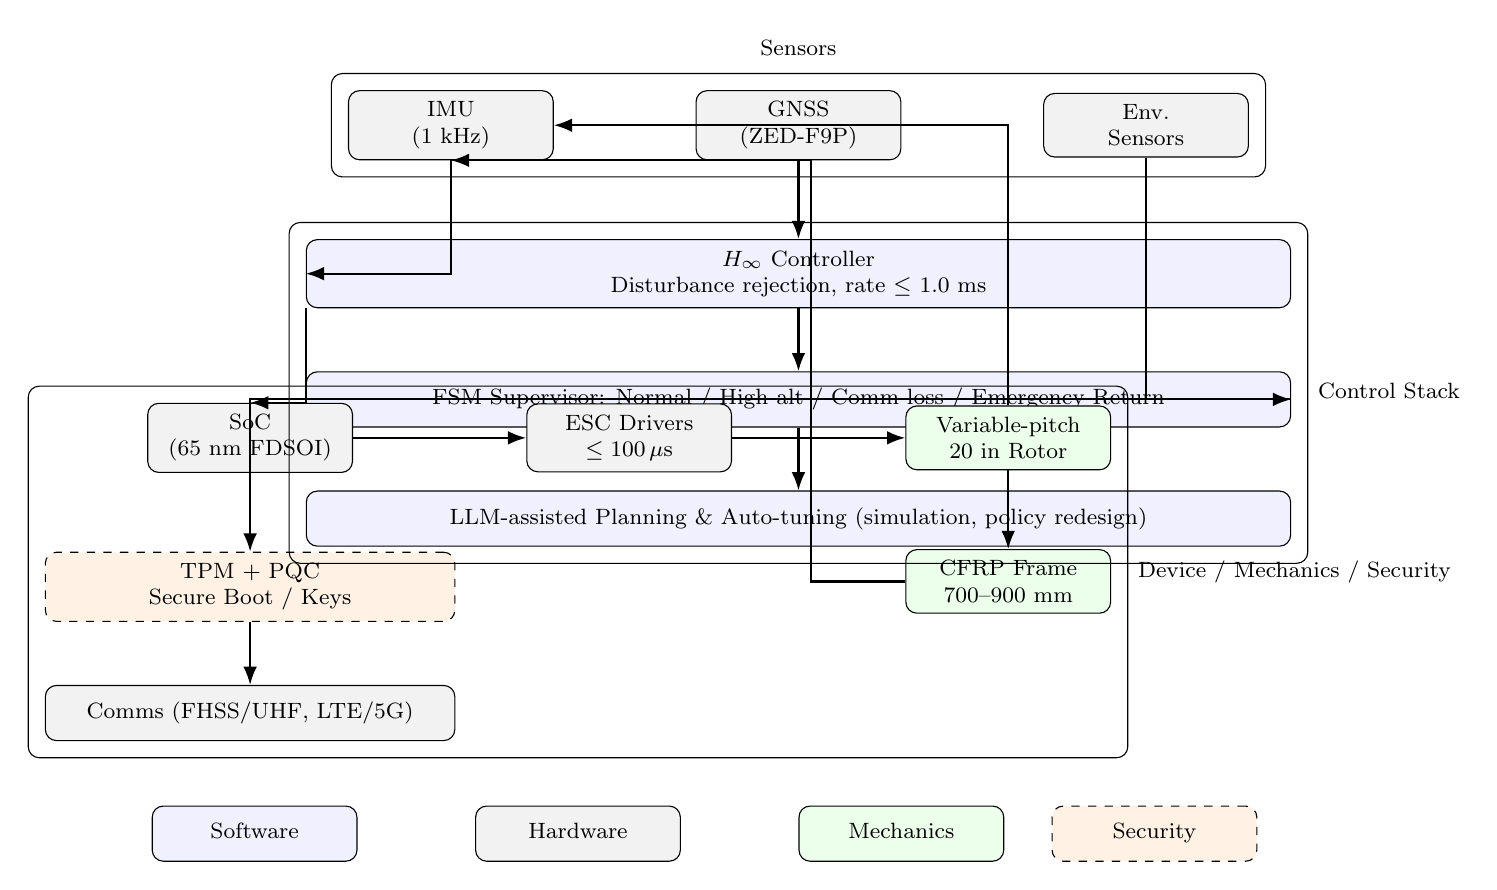
\begin{tikzpicture}[
    font=\footnotesize,
    node distance=8mm and 12mm,
    box/.style={draw, rounded corners, align=center, inner sep=4pt, minimum width=2.6cm, minimum height=7mm},
    hw/.style={box, fill=gray!10},
    sw/.style={box, fill=blue!6},
    mech/.style={box, fill=green!8},
    sec/.style={box, fill=orange!10, dashed},
    arrow/.style={-Latex, thick},
    grp/.style={draw, rounded corners, inner sep=6pt}
]

% ===== Sensors =====
\node[hw] (imu) {IMU\\(1 kHz)};
\node[hw, right=18mm of imu] (gps) {GNSS\\(ZED-F9P)};
\node[hw, right=18mm of gps] (env) {Env.\\Sensors};

% ===== H-infty control (inner loop) =====
\node[sw, below=10mm of gps, minimum width=12.5cm] (hinf) {$H_\infty$ Controller\\
Disturbance rejection, rate $\leq$ 1.0 ms};

% ===== FSM / LLM =====
\node[sw, below=8mm of hinf, minimum width=12.5cm] (fsm) {FSM Supervisor: Normal / High-alt / Comm-loss / Emergency Return};
\node[sw, below=8mm of fsm, minimum width=12.5cm] (llm) {LLM-assisted Planning \& Auto-tuning (simulation, policy redesign)};

% ===== Hardware stack (row) =====
\node[hw, below left=12mm and -6mm of hinf] (soc) {SoC\\(65 nm FDSOI)};
\node[hw, right=22mm of soc] (esc) {ESC Drivers\\$\leq 100\,\mu$s};
\node[mech, right=22mm of esc] (vp) {Variable-pitch\\20 in Rotor};

% ===== Mechanics / Security / Comms =====
\node[mech, below=10mm of vp] (frame) {CFRP Frame\\700--900 mm};
\node[sec, below=10mm of soc, minimum width=5.2cm] (secblk) {TPM + PQC\\Secure Boot / Keys};
\node[hw, below=8mm of secblk, minimum width=5.2cm] (comms) {Comms (FHSS/UHF, LTE/5G)};

% ===== Group boxes =====
\node[grp, fit=(imu)(gps)(env), label=above:{\strut Sensors}] (gSensors) {};
\node[grp, fit=(hinf)(fsm)(llm), label=right:{\strut Control Stack}] (gCtrl) {};
\node[grp, fit=(soc)(esc)(vp)(frame)(secblk)(comms),
      label=right:{\strut Device / Mechanics / Security}] (gHW) {};

% ===== Connections =====
\draw[arrow] (imu.south) |- (hinf.west);
\draw[arrow] (gps.south) -- (hinf.north);
\draw[arrow] (env.south) |- (fsm.east);

\draw[arrow] (hinf.south) -- (fsm.north);
\draw[arrow] (fsm.south) -- (llm.north);

\draw[arrow] (hinf.south west) |- (soc.north);
\draw[arrow] (soc.east) -- (esc.west);
\draw[arrow] (esc.east) -- (vp.west);
\draw[arrow] (vp.south) -- (frame.north);

\draw[arrow] (fsm.east) -| (secblk.north);
\draw[arrow] (secblk.south) -- (comms.north);

% Feedback
\draw[arrow] (frame.west) -| ++(-12mm,0) |- (imu.south);
\draw[arrow] (vp.north) |- (imu.east);

% ===== Legend (centered, no overlap) =====
\path (gHW.south) ++(0,-6mm) coordinate (leg);
\node[box, fill=blue!6,  anchor=north east] (lg1) at ($(leg)+(-28mm,0)$) {\strut Software};
\node[box, fill=gray!10, anchor=north]      (lg2) at (leg)               {\strut Hardware};
\node[box, fill=green!8, anchor=north west] (lg3) at ($(leg)+(28mm,0)$)   {\strut Mechanics};
\node[box, fill=orange!10, dashed, anchor=north west] (lg4)
      at ($(lg3.north east)+(6mm,0)$) {\strut Security};

\end{tikzpicture}%
}
\caption{SkyEdge system architecture (two-column figure). The three-layer control stack ($H_\infty$, FSM, LLM) integrates with sensors, a secure device stack (SoC, TPM/PQC, comms), and variable-pitch mechanical design.}
\label{fig:sysarch}
\end{figure*}

% ===================== Fig.2 (ONE column) =====================
\begin{figure}[t]
\centering
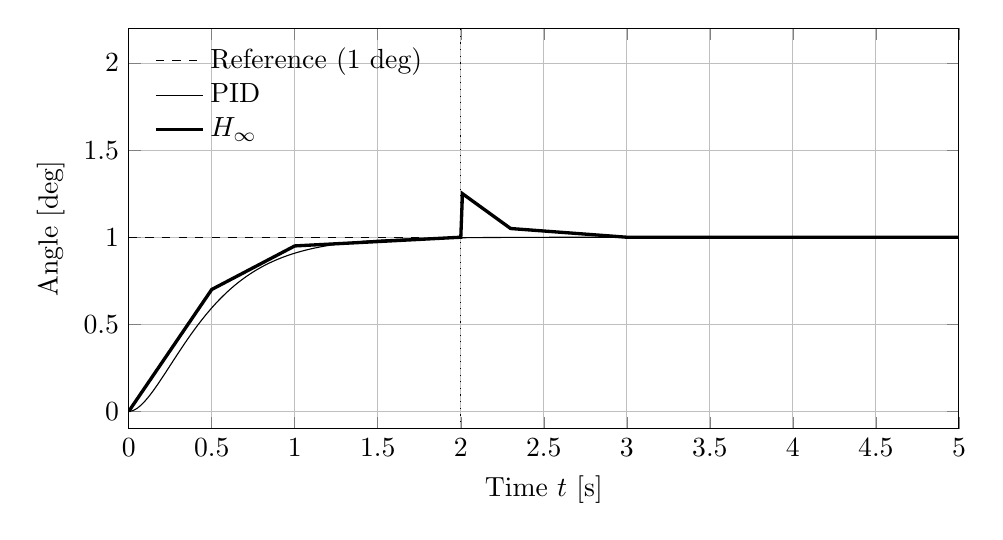
\begin{tikzpicture}
\begin{axis}[
    width=\columnwidth, height=0.55\columnwidth,
    xmin=0, xmax=5, ymin=-0.1, ymax=2.2,
    xlabel={Time $t$ [s]}, ylabel={Angle [deg]},
    grid=both,
    legend style={at={(0.02,0.98)},anchor=north west,draw=none,fill=none},
    legend cell align={left},
    ytick distance=0.5, xtick distance=0.5
]
% reference
\addplot[dashed] coordinates {(0,1) (5,1)};
\addlegendentry{Reference (1 deg)}

% PID(※ 角括弧あり!)
\addplot[smooth,domain=0:5,samples=200] {1 - exp(-4*x)*(1 + 4*x)};
\addlegendentry{PID}

% H-infinity response with gust at t=2 s
\addplot[very thick] coordinates
{(0,0) (0.5,0.7) (1,0.95) (2,1.0) (2.01,1.25) (2.3,1.05) (3,1.0) (5,1.0)};
\addlegendentry{$H_\infty$}

% gust marker
\draw[dotted] (axis cs:2,-0.1) -- (axis cs:2,2.2);
\end{axis}
\end{tikzpicture}
\caption{Step tracking with a sudden gust. The $H_\infty$ controller yields smaller overshoot and faster recovery than PID when a $+15\%$ gust hits at $t=2$ s.}
\label{fig:step}
\end{figure}

% ===================== Fig.3 (ONE column) =====================
\begin{figure}[t]
\centering
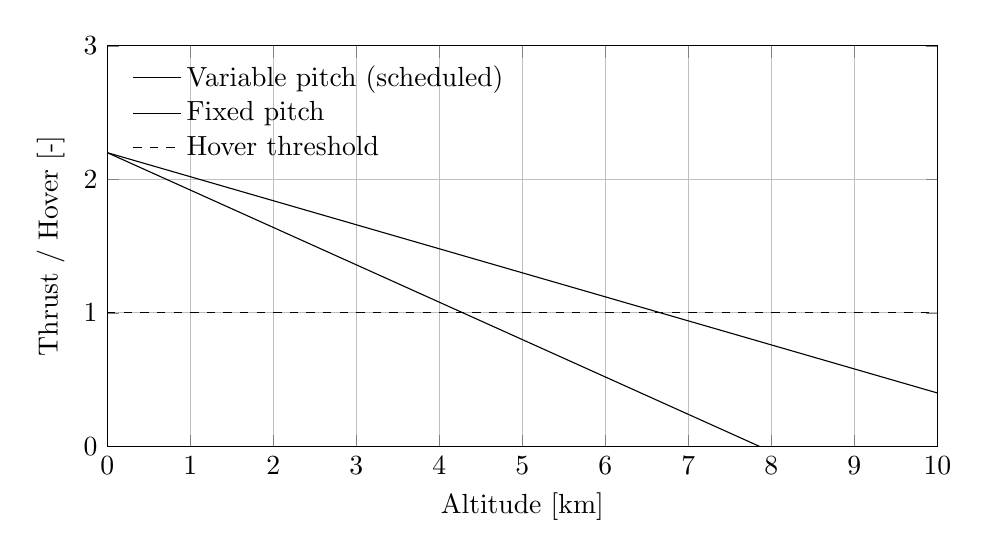
\begin{tikzpicture}
\begin{axis}[
    width=\columnwidth, height=0.55\columnwidth,
    xmin=0, xmax=10, ymin=0, ymax=3,
    xlabel={Altitude [km]}, ylabel={Thrust / Hover [-]},
    grid=both, legend style={at={(0.02,0.98)},anchor=north west,draw=none,fill=none},
    legend cell align={left}
]
\addplot[smooth,domain=0:10,samples=200] {2.2 - 0.18*x};      % variable pitch (scheduled)
\addlegendentry{Variable pitch (scheduled)}
\addplot[smooth,domain=0:10,samples=200] {2.2 - 0.28*x};      % fixed pitch
\addlegendentry{Fixed pitch}
\addplot[dashed] coordinates {(0,1) (10,1)};                   % hover threshold
\addlegendentry{Hover threshold}
\end{axis}
\end{tikzpicture}
\caption{Thrust margin vs. altitude. Pitch scheduling maintains margin above $1$ up to 10 km, while a fixed-pitch rotor loses margin.}
\label{fig:margin}
\end{figure}

% ===================== Fig.4 (ONE column) =====================
\begin{figure}[t]
\centering
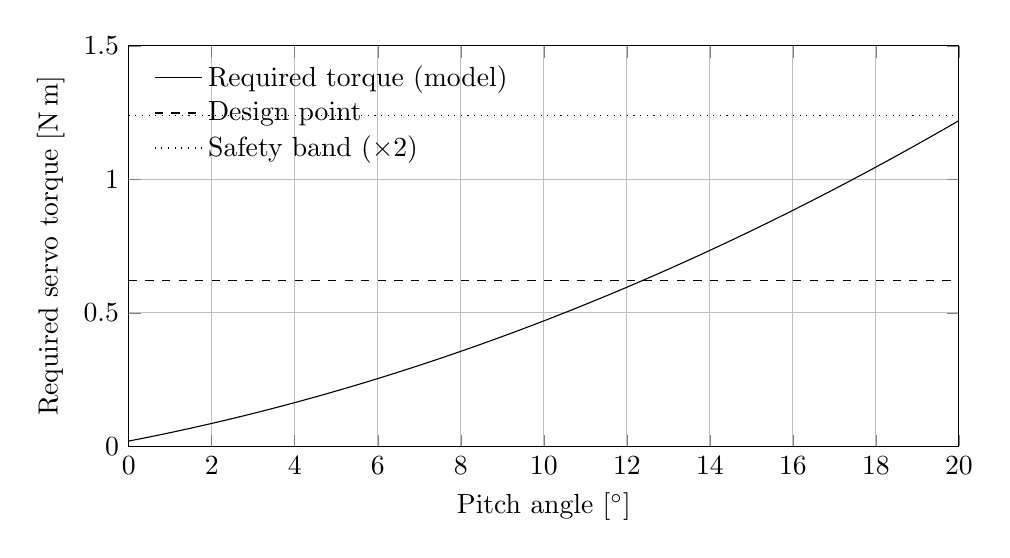
\begin{tikzpicture}
\begin{axis}[
    width=\columnwidth, height=0.55\columnwidth,
    xmin=0, xmax=20, ymin=0, ymax=1.5,
    xlabel={Pitch angle [\si{\degree}]}, ylabel={Required servo torque [N\,m]},
    grid=both, legend style={at={(0.02,0.98)},anchor=north west,draw=none,fill=none},
    legend cell align={left}
]
\addplot[smooth,domain=0:20,samples=200] {0.02 + 0.03*x + 0.0015*x*x};
\addlegendentry{Required torque (model)}
\addplot[dashed] coordinates {(0,0.62) (20,0.62)};
\addlegendentry{Design point}
\addplot[dotted] coordinates {(0,1.24) (20,1.24)};
\addlegendentry{Safety band ($\times 2$)}
\end{axis}
\end{tikzpicture}
\caption{Servo torque vs. pitch angle for the variable-pitch mechanism. The design point \SI{0.62}{N\,m} leaves a safety margin of $\times 2$.}
\label{fig:torque}
\end{figure}

% ===================== Fig.5 (ONE column) =====================
\begin{figure}[t]
\centering
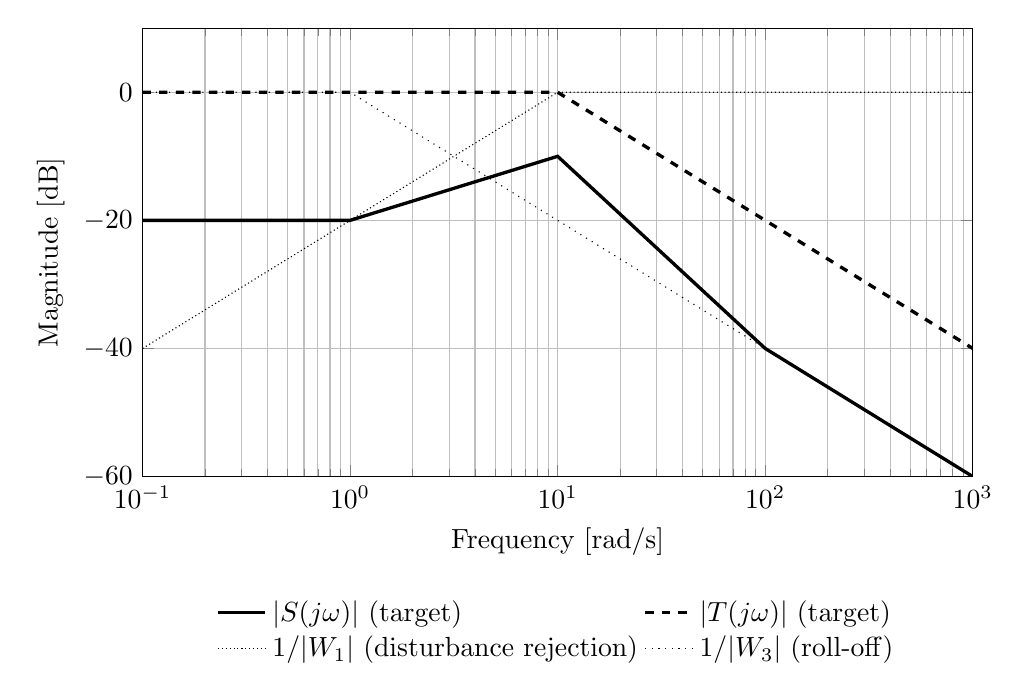
\begin{tikzpicture}
\begin{semilogxaxis}[
    width=\columnwidth, height=0.6\columnwidth,
    xmin=1e-1, xmax=1e3, ymin=-60, ymax=10,
    xlabel={Frequency [rad/s]}, ylabel={Magnitude [dB]},
    grid=both,
    legend style={at={(0.5,-0.25)},anchor=north,draw=none,fill=none},
    legend columns=2,                 % ← 2列で省スペース
    legend cell align={left}
]
\addplot[very thick] coordinates {(0.1,-20) (1,-20) (10,-10) (100,-40) (1000,-60)};
\addlegendentry{$|S(j\omega)|$ (target)}
\addplot[dashed, very thick] coordinates {(0.1,0) (1,0) (10,0) (100,-20) (1000,-40)};
\addlegendentry{$|T(j\omega)|$ (target)}
\addplot[densely dotted] coordinates {(0.1,-40) (1,-20) (10,0) (100,0) (1000,0)};
\addlegendentry{$1/|W_1|$ (disturbance rejection)}
\addplot[dotted] coordinates {(0.1,0) (1,0) (10,-20) (100,-40) (1000,-60)};
\addlegendentry{$1/|W_3|$ (roll-off)}
\end{semilogxaxis}
\end{tikzpicture}
\caption{Frequency-domain intuition for $H_\infty$ design: low $|S|$ at low--mid frequency (disturbance rejection) and low $|T|$ at high frequency (noise/roll-off).}
\label{fig:weights}
\end{figure}

% =============================================================
\section{Device Integration}
A domestic \SI{65}{nm} FDSOI SoC runs the stack with deterministic scheduling; LDMOS ESC drivers achieve sub-\SI{100}{\micro\second} latency; sensors include 1~kHz IMU, ZED-F9P GNSS, and environmental probes. Communication redundancy: FHSS/UHF primary, LTE/5G secondary; automatic failover $<200$~ms with key rollover. Estimated BOM per prototype: \SI{596700}{JPY}; thermal design adds conformal coating and vented enclosure for low-pressure operation.

% =============================================================
\section{Evaluation Plan and KPIs}
\subsection{Wind-Tunnel (WT)}
Gust steps $+15\%$ at $t=2$~s and sinusoidal turbulence (Kaimal spectrum). KPIs: overshoot $<15\%$, $t_{2\%}<0.8$~s, peak effort $<80\%$ of actuator, gain/phase margins $>8$~dB/\SI{45}{\degree}.

\subsection{Thermal-Vacuum (TVAC)}
$-40$ to $+60^\circ$C at equivalent 8--10~km pressure. KPIs: deadline miss rate $<10^{-6}$, ESC derating $<10\%$, reboot-free 4~h dwell.

\subsection{RF Robustness}
FHSS under wideband noise SIR $-5$~dB and tone jammers. KPIs: packet loss $<1\%$, command latency $<30$~ms, LTE/5G failover $<200$~ms with uninterrupted crypto.

\subsection{Fault Injection}
Sensor bias $0.6^\circ$ and ESC dropout. KPIs: detection $<0.5$~s, attitude error $<5^\circ$ for 2~s, graceful FSM transition.

\subsection{Flight Trials}
Step winds \SI{8}{m/s} at 2~km, climbs to 6, 8, 10~km (progressive), with power/thermal logging. Acceptance: thrust margin $>1.0$ at each plateau, control stability without pilot override.

% =============================================================
\section{Limitations and Ethics}
We assume rigid body and small-angle linearization near hover; aggressive maneuvers at 10~km are out-of-scope. PQC increases bandwidth/compute; we mitigate by session-based keying. Operations will follow airspace regulations and geofencing to minimize risk to people and wildlife.

% =============================================================
\section{Applications and Use-Cases}
SkyEdge is designed as a versatile platform, enabling multiple mission
profiles across defense, civil, and environmental domains. By sustaining
robust high-altitude operation with integrated security, several
use-cases become feasible:  

\subsection{Disaster Communications}
In post-earthquake or tsunami scenarios, terrestrial communication
infrastructure often fails. SkyEdge can provide airborne relay links
over 50--100 km radius, supporting LTE/5G backhaul and secure emergency
broadcasts.  

\subsection{Border Surveillance}
Persistent flights at 8--10 km enable wide-area monitoring of remote
border regions. Integration of EO/IR payloads facilitates intrusion
detection, with secure telemetry preventing adversarial spoofing or
jamming.  

\subsection{Environmental Monitoring}
The platform can carry sensors for volcanic activity, glacier melt,
forest fire detection, or greenhouse-gas measurements. The variable-pitch
system maintains efficiency during long-endurance sampling missions
under low-density air.  

\subsection{Defense and ISR Operations}
SkyEdge supports intelligence, surveillance, and reconnaissance (ISR)
missions in contested airspace. With $H_\infty$-based gust rejection and
secure comms hardened by PQC, the platform sustains operation even under
GPS jamming or RF interference.  

% =============================================================
\section{Limitations and Ethics}
Despite its technical contributions, SkyEdge must be deployed within
ethical and regulatory boundaries.  

\subsection{Airspace Regulation}
Operation at 8--10 km intersects controlled civil airspace. Compliance
with ICAO and national aviation regulations is mandatory, requiring
coordination with air-traffic authorities for flight corridors and
emergency descent procedures.  

\subsection{Privacy and Civil Use}
Persistent surveillance raises privacy concerns. To prevent misuse,
mission profiles for civil deployment should enforce strict geofencing,
data minimization, and encryption of sensitive imagery.  

\subsection{Export and Security Controls}
The integration of post-quantum cryptography may fall under export
regulations (e.g., ITAR/EAR). Clear compliance pathways are required
before international deployment.  

\subsection{Ethical Deployment Guidelines}
To align with humanitarian priorities, SkyEdge missions should
prioritize disaster relief, environmental safety, and public benefit.
Use in fully autonomous lethal applications is beyond the intended
scope. Human oversight must remain central to mission authorization and
system reconfiguration.  

% =============================================================
\section{Conclusion}
SkyEdge combines $H_\infty$ control with altitude scheduling, domestic secure hardware, and variable-pitch mechanics to sustain high-altitude flight with security guarantees. The provided models, synthesis settings, timing/crypto pipeline, and KPI-based plan aim to ease reproduction and certification-oriented testing.

% ---------- References ----------
\balance
\bibliographystyle{IEEEtran}
\begin{thebibliography}{99}
\bibitem{zhou1996robust} K. Zhou, J. C. Doyle, and K. Glover, \emph{Robust and Optimal Control}. Prentice Hall, 1996.
\bibitem{nasahelios} NASA, ``Helios Prototype UAV,'' NASA Facts, 2003.
\bibitem{jaxaHAPS} JAXA, ``High Altitude Platform Station (HAPS) Research,'' 2020.
\bibitem{dji2022} DJI, ``Matrice 300 RTK Specifications,'' DJI, 2022.
\bibitem{pqcrypto2022} NIST, ``Post-Quantum Cryptography Standardization,'' 2022.
\bibitem{mpc2021} F. Borrelli et al., ``Model Predictive Control for Aerial Vehicles,'' \emph{IEEE Control Systems Magazine}, 2021.
\bibitem{rluav2022} H. Zhu et al., ``Reinforcement Learning for UAV Flight Control under Disturbances,'' in \emph{IROS}, 2022.
\end{thebibliography}

\end{document}
